\chapter{Dynamic Instrumentation Using Code Analysis And Transformation For Detailed GPU Communication Analysis}
This chapter describes how the instrumentation to generate trace data is realized. Goal of the instrumentation is to modify the original source so it generates data at run time that can be used to identify communication between CTAs in an application. As global memory is the only address space allowing side-effects beyond kernel kernel completion boundaries (KCB), global memory operations are the target of the instrumentation. Data is generated by creating a trace record every time a global memory operation is performed.  Before a detailed explanation of the steps, an overview of the involved components is given. The instrumentation happens during the build of the program and is handled in Clang and LLVM. They are used to insert code and functions for the data generation.

Communication across BSP steps, honouring the guarantees CUDA's execution model gives, is not bound to any timing or ordering during the execution of a single compute kernel. Negative performance impacts by the instrumentation is therefore tolerated, 
because in a well-written program the negative impact does not impede the correctness.

As libraries present external code not in source or LLVM IR, code using libraries can't be reliably instrumented.

\section{Trace Setup}
Figure \ref{overview} shows at which points the original application is extended. The instrumented kernel generates data, which is consumed by a thread running on the host. This consumer thread forwards the data to a 
storage, in this case a simple file. Stream callbacks are used to encapsulate the kernel
between two functions controlling the trace consumer. This guarantees isolated traces for every kernel in a stream.
CUDA streams allow concurrent execution of kernels and DMA data movement on one device.
A stream also allows executing multiple kernels at the same time, as long as resources are available. Multiple kernels simultaneously executed using the same buffer lead to unordered data that is not clearly assigned to a stream or kernel. Post-morten separation of data is infeasible. Multiple consumer threads, each managing one stream and private buffers and storages for each of them resolve this issue. Interaction between streams can be tracked by cross-referencing the stream files in the later analysis of the data.
\begin{figure}[t]
	\centering
	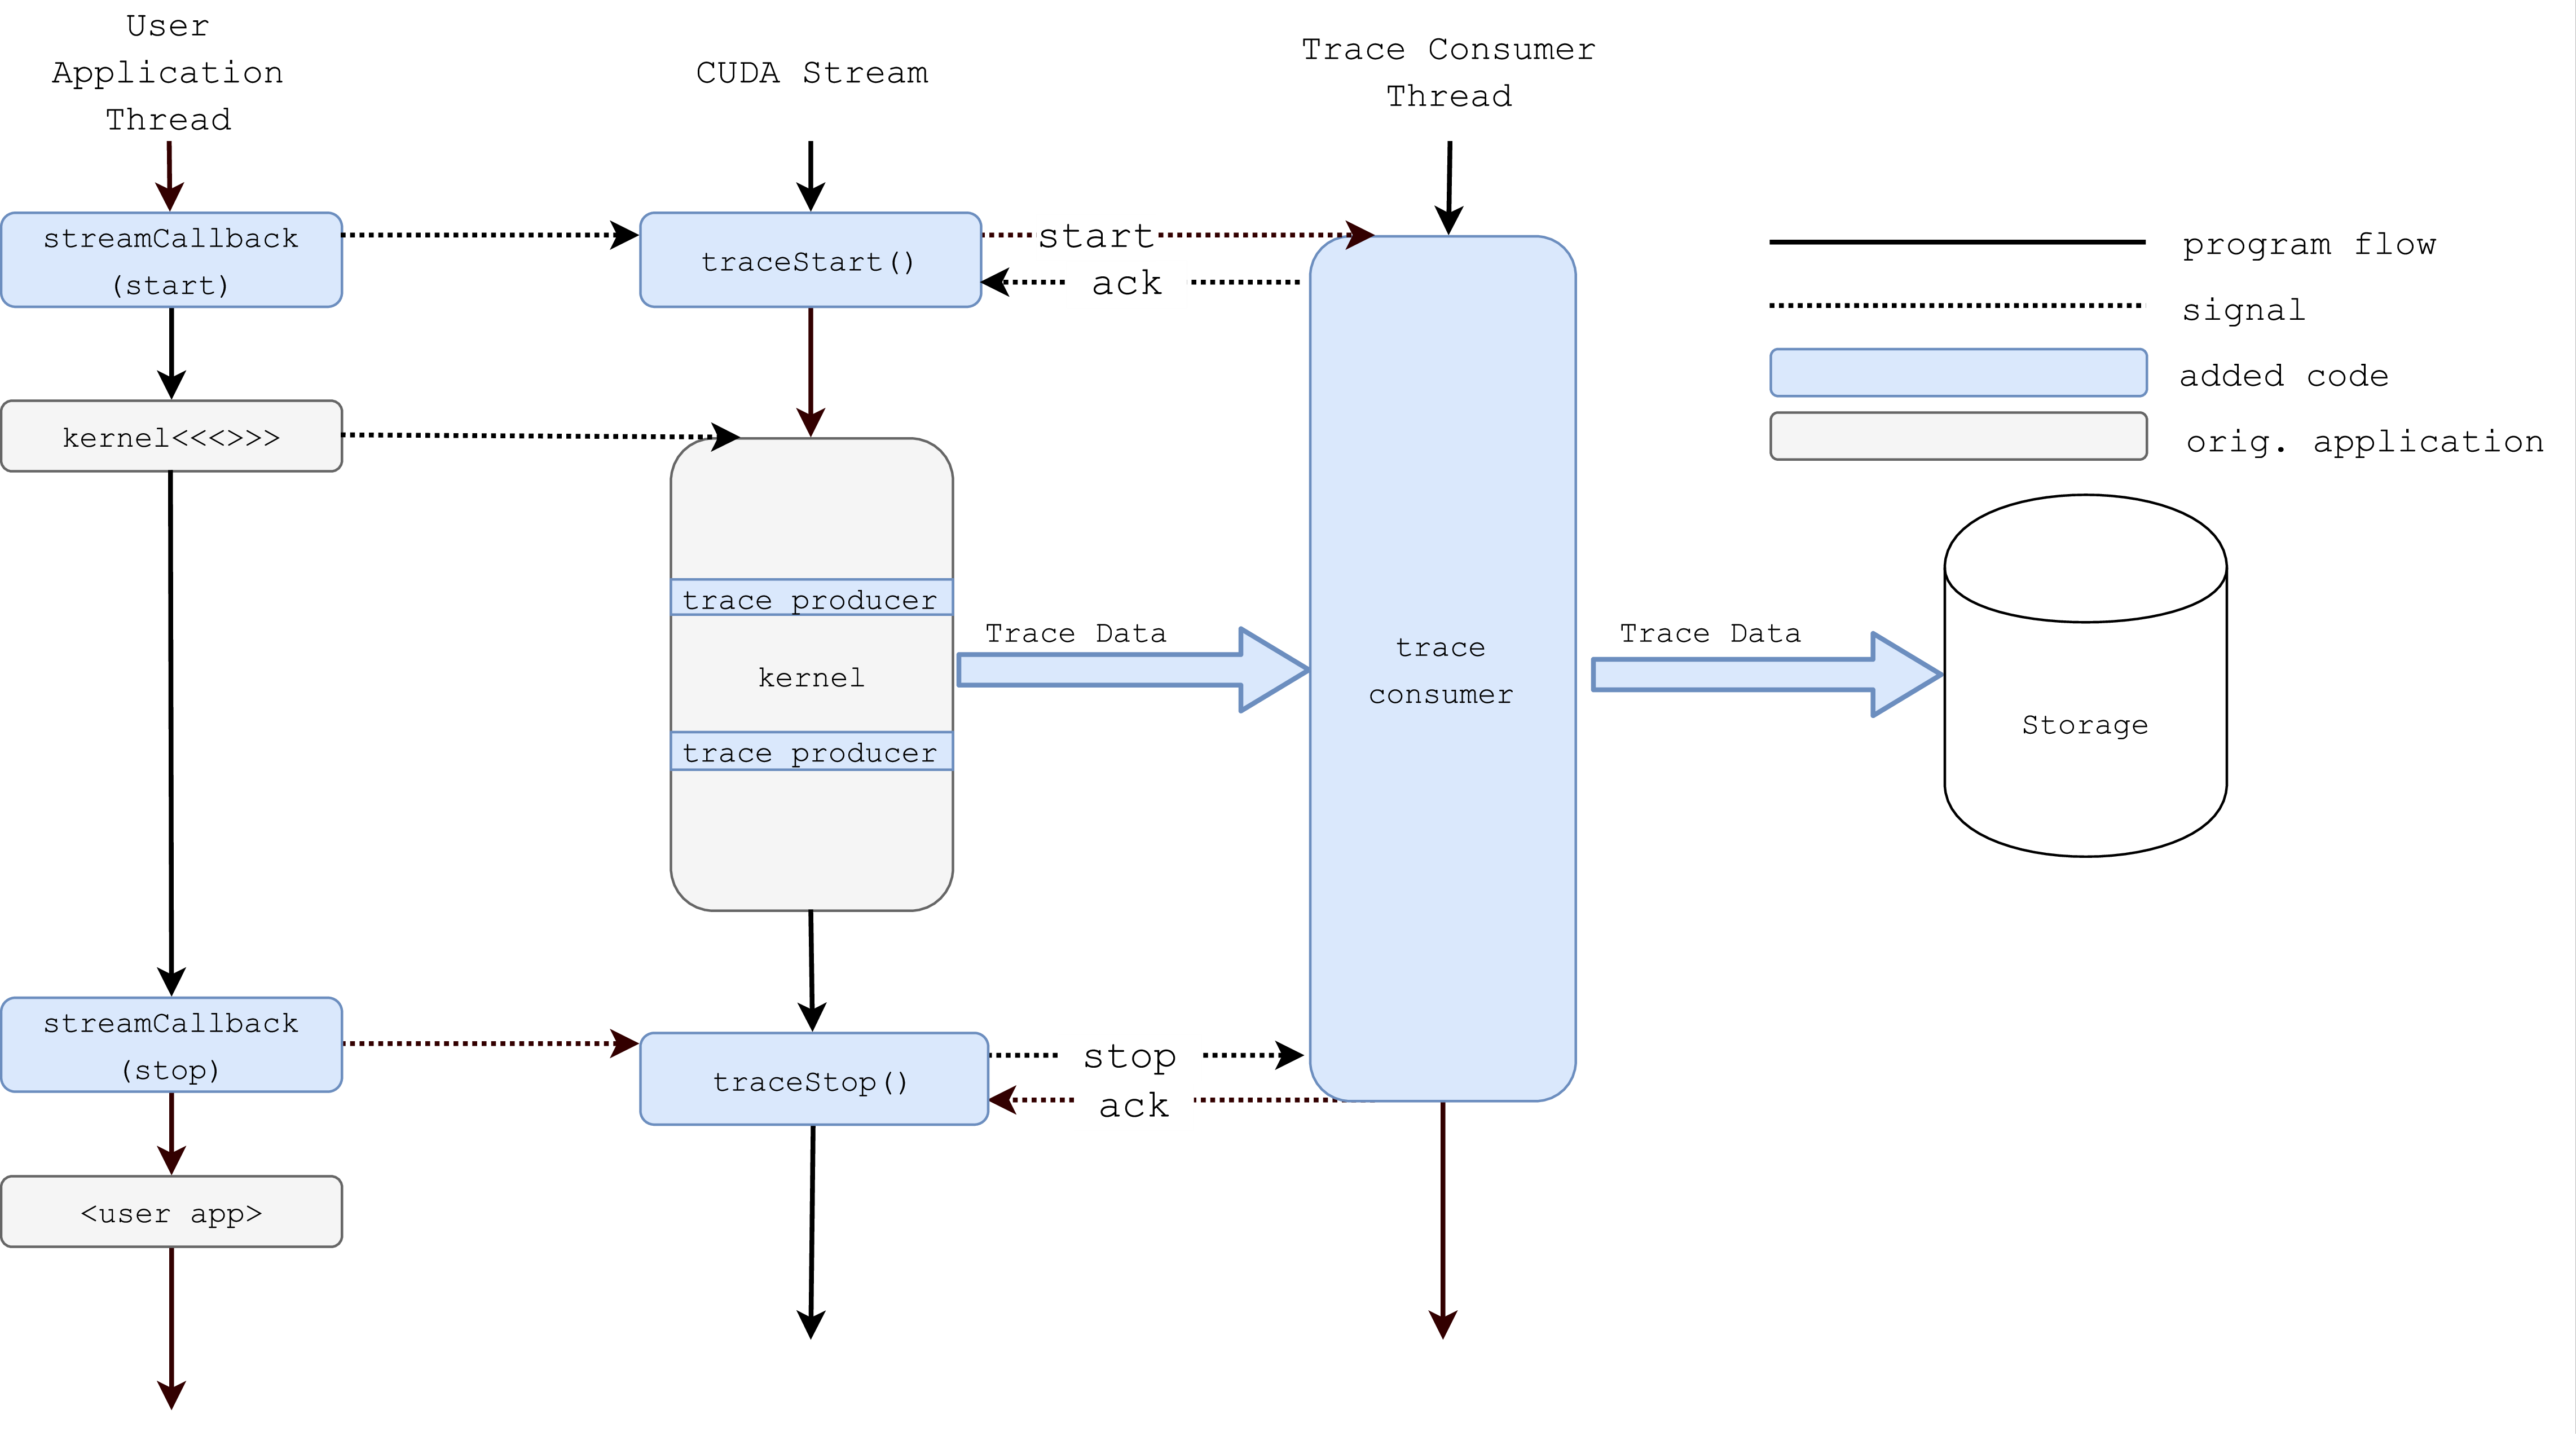
\includegraphics[width=\textwidth]{overview}
	\caption{Structure of an instrumented application. Segments added during instrumentation are highlighted in blue.}
	\label{overview}
\end{figure}


\subsection{Build Process}
Host side modification happens in a Clang front-end plugin. This plugin extends kernel and function declarations and definitions and includes functions used by the trace. This generates a new file that is used instead of the original source . The instrumentation to trace memory operations in the kernel is done by an LLVM optimization pass and happens during the compilation of the file augmented by Clang. After compilation and instrumentation, the created object files are linked together with the rest of the application and object files used by the trace.
Clangs task is detailed is section \ref{sec:impl:clang}, LLVMs process is elaborated in section \ref{impl:llvm} and section \ref{sec:prodcons} covers details on how data is buffered and transferred from device to host at kernel run time.
\begin{figure}[t]
	\begin{lstlisting}[style=C]
	|32 bit |4 bit   |28 bit |64 bit |64 bit        	  |
	|191 160|159  156|155 128|127  64|63   32|31  16|15  0|
	|SMID   |Type    |Size   |Address|CTA.x  |CTA.y |CTA.z|	\end{lstlisting}
	\caption{Trace record format}
	\label{trace rec}
\end{figure}
\begin{figure}[t]
	\begin{lstlisting}[style=C]
	<size of one record, in bytes> //stored in a single byte
	<kernel name> // name of kernel, followed by LF
	<records> // all trace records, as one binary blob
	000000000000000000000000 // EOT
	<kernel name>
	<records>
	000000000000000000000000
	<EOF>	\end{lstlisting}
	\caption{Trace file format}
	\label{trace file}
\end{figure}
\subsection{Trace Format}
A trace record consists of 192 bits of data as detailed in code snippet \ref{trace rec}, stored in LSB order. It contains the executing SM, CTA ID, size of the data type, type of memory operation and the operation's address. The record format allows to track the interactions between CTAs across KCBs on a per-address basis. Which subsets of the interactions contain actual communication is explained in chapter \ref{eval}.
The format of a complete trace file is shown in listing \ref{trace file}. The first byte in a file is the record length, followd by a \verb|LF|. The next line contains the
traced kernel's name. Because all records have the same size, they are stored without a separator. End of trace (EOT) for a kernel is marked by a record consisting of only zeroes. The next line contains the name of the follow-up kernel.




\section{Source to Source Compilation in Clang}\label{sec:impl:clang}
The first instrumentation step extends the host code and adds includes that are used by the kernel. It uses a Clang front-end plugin to transform a file and generate a new, augmented source code that is then used in the build process. The plugin uses the \verb|ASTVisitor|
pattern in clang's API to traverse statements and declarations of interest. After the AST modification, a new file is written and two
headers are added.

\begin{itemize}
	\item \verb|TraceUtils.h| contains buffer and stream management, trace consumer control and storage.
	\item \verb|DeviceUtils.h| contains \verb|__device__| functions used for the trace. The file is included in all
	files containing kernel code because the following LLVM optimization pass will create calls to these functions in the original kernel.
\end{itemize}

\paragraph{AST Declarations} contain kernel and \verb|__device__| function declarations. They are extended with the following arguments:
\begin{itemize}
	\item \textbf{Reservation Index Array:} Array of indices for buffer space reservation. Because each buffer is segmented into various bins,
		each bin needs it's own index.
	\item \textbf{Acknowledgement Index Array:} Array of indices for write acknowledgements. Because each buffer is segmented into various bins,
	each bin needs it's own index.
	\item \textbf{Buffer Pointer:} Base pointer of the buffer.
	\item \textbf{Bin Size:} Max. number of elements per bin.
	\item \textbf{Bin Count:} Number of available bins.
\end{itemize}
The mentioned bins are a logical division of buffer space due to reasons explained in \ref{sec:prodcons}. They are not be mistaken 
for the private buffers of each stream! Each stream buffer is divided into bins.

\paragraph{AST Statements} contain the calls kernels and \verb|__device__| functions. The augmentation of the latter is trivial. The kernel's trace arguments are passed to the function. The former however needs more manipulation.

First, the stream is extracted from the kernel parameters. Two statements are inserted before the kernel call. The first one allocates stream buffers, creates the storage and spawns the consumer thread in a waiting state. This only happens once per stream. Next,1 the function starting the consumer thread  is issued to the stream, using \verb|cudaStreamAddCallback()|. Now the kernel call is extended using the buffers allocated for this stream. After the call the function stopping the trace consumer is issued to the stream. It guarantees that
the buffered data is consumed and stored before starting another trace.
An explicit stream synchronization is therefore not necessary.

\section{Code Transformation in LLVM}\label{impl:llvm}
Instrumenting the application to generate trace data for global memory operations on the GPU happens inside an LLVM IR optimisation pass. The original source is analysed and instrumented at the locations of loads, stores and atomic operations targeting global memory, so that during the execution data is generated. Before the call kernel

Global memory is the only address space of CUDA in which side effects that are visible across kernel completion boundaries are possible. These side effects can carry information from a kernel to another and so memory operations using this address space need instrumentation. Finding loads and stores targeting global memory is not trivial in LLVM IR. Clang performs lowering of all memory access operations during the generation of LLVM IR and in the process eliminates the address space information at location of the memory operation. An example for the lowering is displayed in listing \ref{lowering}. The \verb|getelementptr| instruction is used for address calculation, for example to access a specific element in an array. However, before this an \verb|addrspacecall| casts the pointer form address space 3 (shared memory) to address space 0 (generic address space). The pointer used in the \verb|store| instruction in line two does not contain information about its address space. This lack of information means the LLVM pass can not visit loads and stores exclusively to determine the address space and a more complex approach is necessary.
 
PTX does not necessarily need address space information for a memory operation since it can be resolved dynamically during runtime. While PTX has distinct load (\verb|ld|) and store (\verb|st|) instruction for
each address space, a generic version is also available. This generic instruction maps to global memory, if
it does not fit into a window for the other address spaces \cite{ptx isa}. This lookup however comes at the cost of a minor performance decrease \cite{infer-pass}. So, while beneficial it is not necessary to
have the address space information to build a correct application. For the tracing process, however, we need to have this information to prevent the generation of trace data for parts of the address space that are not interesting for this work.

\begin{figure}
	\begin{lstlisting}[style=C]
%arrayinx1 = getelementptr inbounds (float, float* addrspacecast (float addrspace(3)* @_ZZ5saxpyfPfS_iPlS0_E2_x to float*), i64 0, i64 2)
store float 1.000000e+00, float* %arrayinx1
	\end{lstlisting}
	\caption{Example for address space lowering in LLVM IR}
	\label{lowering}
\end{figure}

There is an experimental LLVM optimizer pass which tries to infer the address space by analysing the steps that have been introduced by the lowering. However, it works on a function scope which is not sufficient for our purposes. Address space information  might not be existing in the function argument because of lowering of the argument previous to the function call. And due to the pass' function scope, information on the calling context is not available. Because the pass can fall back to the generic address space,
it is not critical if the address space cannot be determined reliably. This is not sufficient for the needs of this work because the address space information needs to be definite.
Therefore an  analysis is performed, that generates definitive information, whether a memory access targets
global memory or not. If generating this information is not possible, the pass fails. The reason for an unsuccessful execution is  explained in section \ref{pa}, after more details of the actual analysis have been explained.

LLVM widest analysis scope is 'Module', which roughly corresponds to one translation unit in C. Interactions of the original source that reach beyond this Module scope cannot be analysed, and therefore not instrumented.

\subsection{Address Space Analysis}\label{pa}
The basic principle of this analysis rests on the limited number of sources in 
a kernel, where a global address space pointer can be obtained from.
\begin{itemize}
	\item direkt kernel parameters
	\item indirekt kernel parameters (struct etc.)
	\item global variables
	\item pointer type load from global memory
\end{itemize}
Collecting base pointers form all these sources provides starting points for a sparse analysis of the program,
because only memory operations that are part of def-use chains rooting in these base pointers, can be a candidate for instrumentation.

%	\begin{defi}
%	$	MOp = \{\textrm{LoadInst, StoreInst, atomicInst}\} $
%	\end{defi}
%	\begin{defi}
%	$   POp = \{ \textrm{LoadInst of Type Ptr, GetElementPtr, CastInst, Arg of CallInst} \} $
%	\end{defi}
%	\begin{defi}
%	$	NMOp = \{inst : inst \notin POp, inst \notin MOp\}$
%	\end{defi}


%	\centering
%	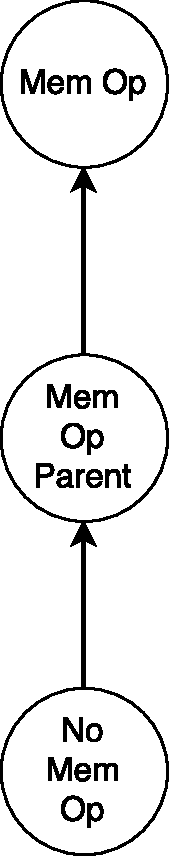
\includegraphics[height=0.3\textwidth]{lattice}
%	\caption{Property space lattice}
%	\label{ptr-analysis}

The used algorithm performs a 'must'-analysis on the sparse problem space that is represented by the def-use chains created by the SSA form of LLVM IR. Because the the algorithm follows the order of instructions through the program, it can be described as 'flow sensitive'. Function calls are only
analysed if they happen in a 'global-memory context' which in our case means that one of arguments used in the call is a pointer to global memory. This classifies our algorithm as 'context sensitive'.
The property space of the analysis describes sets of instructions in the context of global memory operations that are defined
as following:
\begin{defi}\label{mop}
	$	MOp = \{\textrm{LoadInst, StoreInst, CallInst}\} $
\end{defi}
$MOp$ contains all types of instruction, that are interesting for tracing. During the analysis they are marked for later instrumentation. LLVM maps CUDA's atomic operations to functions, which is why $\textrm{CallInst}$ is part of this set. Of course they are only considered a memory access, if the callee is an atomic function.
\begin{defi}\label{mopp}
	$   POp = \{\textrm{CallInst, GEPInst, CallInst, PHINode, SelectInst}\} $
\end{defi}
$POp$ contains operations that define new SSA variables which can be used in operations interesting for tracing. $CastInst$ because of the lowering  and $GEPInst$ since it is the generic way in LLVM
to perform address arithmetic. Their users need to be visited later. 
$PHINode$ and $SelectInst$ are special cases. Only instructions that resolve pointers and all arguments can be related to a global memory base pointers are a part of this set. The reason for
this is explained in section \ref{patho}.
This set also includes function calls. However, in the case of a function not the return value definition, but the argument passed into the function marked for later analysis. More on the return values of functions in section \ref{patho}.
\begin{defi}\label{nmop}
	$	NMOp = \{inst : inst \notin POp, inst \notin MOp\}$
\end{defi}
$NOp$ contains all instructions that are of no interest for the analysis and are ignored.

To obtain a list of all instruction which require instrumentation, each of the orginal base pointers is handled by Algorithm \ref{anal-algo} to create list of all descendant memory operations of the original by applying the transfer function $f(x)$ to every instruction processed. $f(x)$ classifies each instruction, assigning it to one of the three sets $MOp$, $POp$ or $NOp$. After this, a list with the instructions for tracing of each function has been generated. This algorithm only proves if a memory operation uses a pointer originating from a original base pointer, and therefore uses the same address space, which can be achieved without the need to analyse cycles in the CFG. As a consequence the algorithm always terminates once each relevant instruction is visited. By keeping track of each function that was already visited, recursion is not an issue during the analysis.


\begin{algorithm}[t]
\KwData{orignal pointer}
\KwResult{List of global memory operations based on original pointer }
add original pointer to workstack\;
\While{workstack not empty}{
	get element form workstack\;
	\ForAll{users of element} {
	\tcc{apply tranfer function $f(x)$ to user:}
	\uIf{$type(user) \in MOp$}{
		add user to list for tracing\;
	}\uElseIf{$type(user) \in POp$}{
		add new parent to workstack\;
	}\uElseIf{$type(user) \in NOp$}{
		continue with next user\;
	}

}
}
\caption{How to find global memory operations based on a input pointer}
\label{anal-algo}
\end{algorithm}
\subsubsection{$\phi$-Node Limitations}\label{patho}
Static analysis has some limitations that can cause an unsuccessful address space analysis. This particular issue is caused by the SSA's need to define a new version for a variable each time said variable changes. This results in the need of $\phi$-functions and \verb|select| statements, which is a LLVM IR instruction to handle small \verb|if-else| branches without the need for multiple basic blocks
and a $\phi$-node. Figure \ref{phinodes} shows a minimal code example that can lead to a situation which is not analysable by our static analysis, because it requires resolving pointers to different address spaces at runtime. The code sample on the left creates a situation where a $\phi$-node is required to resolve the edges of the incoming basic blocks. Each of these basic blocks defines a surrogate pointer for \verb|d|. For this example we will call them \verb|ds1| and \verb|ds2|. Based on \verb|ds1| and \verb|ds2| the $\phi$-node defines a pointer \verb|df| that is used for the following operations performed on \verb|d|. Therefore the $\phi$-node resolves which address space \verb|df| points to. 

This is illustrated by graphs on the right hand side of the figure. Every block preceding the $\phi$-node carries an address space, represented by a colour.
The left graph has to resolve different address spaces and therefore the address space for \verb|df| is ambiguous. This leads to an unsuccessful analysis. The right graph shows a special case the implemented pass can resolve by proving that \verb|ds1| and \verb|ds2| both point to the same address space, which concludes that \verb|df|'s address space is definite. The proof is implemented as a table counts how often the analysis pass visits every phi-node. After the analysis is finished the value in the table is compared to the $\phi$-nodes incoming edges. If the counted value and number of edges match the pass proved the special case, otherwise we have ambiguity in the address space of \verb|df|, which leads to aborting the instrumentation pass.

\begin{figure}[t]
		\begin{minipage}{0.35\textwidth}

		\begin{lstlisting}[style=c]
__global__ float *gx;
__shared__ float *sx;
float *d;
if (a > b)
	d = gx;
else 
	d = sx;	\end{lstlisting}
			\end{minipage}\hfill
	\begin{minipage}{0.6\textwidth}
		\centering
		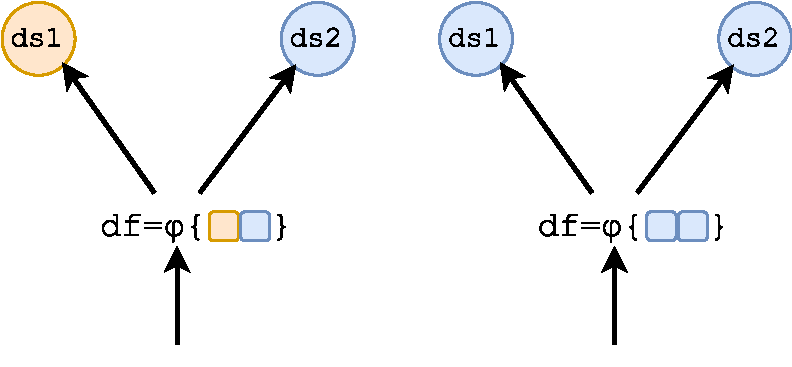
\includegraphics[width=\textwidth]{phinode2}
	\end{minipage}\hfill
	\caption{Example for static analysis limitations. Different colors represent different address spaces. The left graph represents the generic problem case and right graph a special case that is resolvable by the analysis.}
	\label{phinodes}
\end{figure}

\subsubsection{Ambiguous Function Address Space}\label{func-vers}
Another issue is possible ambiguity in the address space of pointers that are passed to functions. To illustrate this issue, figure \ref{func-vers} provides on the left hand side a code sample of a coalescing copy function. CUDA allows calling this device function with pointers to every address space and every combination of address spaces. The kernel on the right hand side then uses the function twice, once to copy data from the global memory into shared memory and a second time to move the data back to the global memory.

Now the instrumentation pass analyses the kernel, finds the first function call and sees that a function is called and the first
parameter is a global memory pointer. It enters the function and marks the \verb|load| instruction for tracing. The pass continues and later finds a call to the same function, enters the function again and this time marks the \verb|store| for tracing, because the pointer
led the pass to it. Now both memory operations are marked as global memory operations and generate trace data, although they are not always used with a global address space pointer. This issue is the reason, our analysis and the added
instrumentation needs to be context sensitive. Potentially, each calling context has unique pattern for tracing.

Context sensitive tracing is implemented using function specialization. During the analysis a table keeps track of each function call, and which of
its arguments belongs to global memory addresses. While gradually working through the initial list of  global memory pointers and tracking their descendants during the analysis, a function call might be visited multiple times and each time a different argument ( and thus different pointer) led the analysis there. These multiples visits form an argument pattern for each function call. After the analysis, all function calls are reduced
to a pattern list for each function. Every pattern contains a combination of arguments that belongs to the global memory address space. A pattern is stored as an unordered tuple with the length corresponding
to number of global memory space pointers and each element is the index in the function's argument list. 
For our example the analysis creates two patterns, $\textbf{\{0\}, \{1\}}$. A third option would be 
 $\textbf{\{0,1\}}$, which would indicate both pointers belong to the global memory address space.
There can be no empty patterns because the analysis would never visit a function call where no global memory pointer is involved.

Now that we know which patterns exists, the original function is cloned once for each pattern. Therefore, the example generates two clones, \verb|copy_0| and \verb|copy_1|. Every created clone is assigned to one function call pattern. Following that, every function call in the created table gets his callee replaced with clone matching the pattern of the call. Based on the call's arguments the analysis is executed again for each function call, now marking the clone's instruction for tracing. During this process, the original function's instructions are removed from the tracing list.

After this process has finished, multiple versions of a function have been created and each of them only creates trace data if they actually required. Specifically, for the example two functions would have been created, one that augments the memory operations on \verb|src| and one for \verb|dst|. The respective calls to \verb|copy| would have been replaced with \verb|copy_0| and \verb|copy_1|. It is possible that more than one parameter is used for tracing.

\begin{figure}[t]
	\begin{minipage}{0.45\textwidth}
		
		\begin{lstlisting}[style=c]
void copy(float* src, float* dst){
	dst[tix] = src[tix];
}\end{lstlisting}
	\end{minipage}\hfill
	\begin{minipage}{0.45\textwidth}
			\begin{lstlisting}[style=c]
__global__ void k (float* gx) {
	__shared__ float* sx;
	copy(gx, sx);
	// kernel does stuff
	copy(sx, gx);
	return;
}\end{lstlisting}
	\end{minipage}\hfill
\begin{minipage}{\textwidth}
	
%	\centering
%	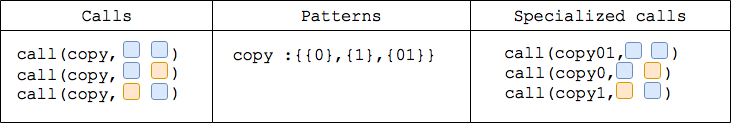
\includegraphics[width=\textwidth]{func-vers}
\end{minipage}\vfill
	\caption{Example for ambiguous function address spaces}
	\label{func-vers}
\end{figure}
\begin{algorithm}[t]
	\KwData{Function Call Table}
	\KwResult{List of global memory operations in cloned functions}
	\ForAll{function calls in table} {
		get argument pattern of call\;
		get or create clone for pattern\;
		replace callee of call with clone\;
		get new argument entrance pointers\;
	}
	\ForAll{new clone pointers} {
		re-analyse all new argument pointers\;
	}
	\caption{Algorithm for function specialization}
	\label{anal-algo}
\end{algorithm}
\subsection{Instrumentation}\label{instru}
The optimizations pass' last step is the actual instrumentation. Some preparation is performed once in every function, before the actual tracing instrumentation takes place.
\begin{enumerate}
	\item Fetch the arguments added by the source-to-source compilation. These arguments contain the trace buffer information.
	\item Add instructions to fetch SMID during runtime. The call 
		\begin{lstlisting}[style=c]
asm("mov.u32 %0, %smid;" : "=r"(sm) )\end{lstlisting}
	copies the value from the special read-only \verb|%smid| register into the register that is accessed by variable \verb|sm|.
	\item Add instructions to calculate trace buffer bin from arguments:
	\begin{lstlisting}[style=c]
nSlots = 1 << PowerOf2OfNumberOfSlots // 1000
slotMask = nSlots - 1 // 0111
bin = slotMask & sm\end{lstlisting}
\end{enumerate}
After the preparation, every instruction marked for tracing in this function is instrumented for tracing by adding a call to the producer function. The producer function was added by the Clang front-end plugin. The call is added before the actual memory operation.
\begin{enumerate}
	\item Get  \verb|Type| descriptor of memory operation. 	\verb|Type| specifies the kind of memory operation specifically and is defined in table \ref{TypeTab}.
	\item Fetch pointer operand that is relevant for tracing
	\item Calculate the size of the memory operation in bytes. Complex data types like \verb|structs| are recursively explored and the total size of the element is calculated.
	\item Insert instructions to generate left-most part of a trace record:
		\begin{lstlisting}[style=c]
64bitDesc = sm << 31
64bitDesc |=  Type
64bitDesc |=  SizeInBytes\end{lstlisting}

	\item Insert call to trace producer function right before the actual memory operation. This function builds the
	last part of the trace record, describing the CTA and then writes the data into the trace buffer selected by \verb|bin|. The details of details of how the data is written into the buffer are explained in section \ref{ondevprod}.
\end{enumerate}
This is performed for every function that requires tracing. After the pass finishes, the application can be built
and linked.
\begin{table}[t]
	\centering
\begin{tabular}{|l|c|}
	\hline 
	Memory Operation & Descriptor \\ 
	\hline 
	Load & 1 << 28 \\ 
	\hline 
	Store & 2 << 28 \\ 
	\hline 
	AtomicAdd & 3 << 28 \\ 
	\hline 
	AtomicSub & 4 << 28 \\ 
	\hline 
	AtomicExch & 5 << 28 \\ 
	\hline 
	AtomicMin & 6 << 28 \\ 
	\hline 
	AtomicMax & 7 << 28 \\ 
	\hline 
	AtomicInc & 8 << 28 \\ 
	\hline 
	AtomicDec & 9 << 28 \\ 
	\hline 
	AtomicCAS & 10 << 28 \\ 
	\hline 
	AtomicAnd & 11 << 28 \\ 
	\hline 
	AtomicOr & 12 << 28 \\ 
	\hline 
	AtomicXor & 13 << 28 \\ 
	\hline 
\end{tabular} 
 \label{TypeTab}
 \caption{Memory operation descriptor table}
\end{table}


\section{Tracing Process}\label{sec:prodcons}
	Many applications have non-deterministic executions, for example no predetermined number of kernel calls because of varying input data. Examples are graph algorithms depending on implementation and data or numerical solvers, which iterate until a
	convergence condition is reached by the residual. Because of this, a static buffer that is filled up once and is cleared at the end of the application does no suffice for reliable and dynamic tracing.
	
	Therefore a producer-consumer queue for the generated trace data between GPU and host is used that ensures the application never runs out of buffer space for the tracing data. The GPU generates the data and the host evacuates full buffers, storing the data.
	The buffer containing the generated data is host-mapped memory, which is separated into several bins. The bins are used to reduce
	pressure on the memory system that is generated by the atomic index accesses of the producer-consumer setup. The number of bins 
	is always a $2^n$ and a scheduled CTA uses the  $n$ least significant bits of the SM's ID it is scheduled on, to select a bin. Therefore the number of bins should be selected as the closest power of two, to the number of SMs.

	Writing the data to disk after they have been cleared from the buffer by the consumer, showed to be a performance critical aspect during the trace. Per default, Linux directs \verb|writes()| to a page cache. Smaller, periodic writes (64Kbyte to 1Mybte) to the disk empirically showed to be more efficient. The author assumes this is caused by overlapping between cache management and queue management.
	
	\subsection{On-Device Producer}\label{ondevprod}
\begin{figure}[t]
	\centering
	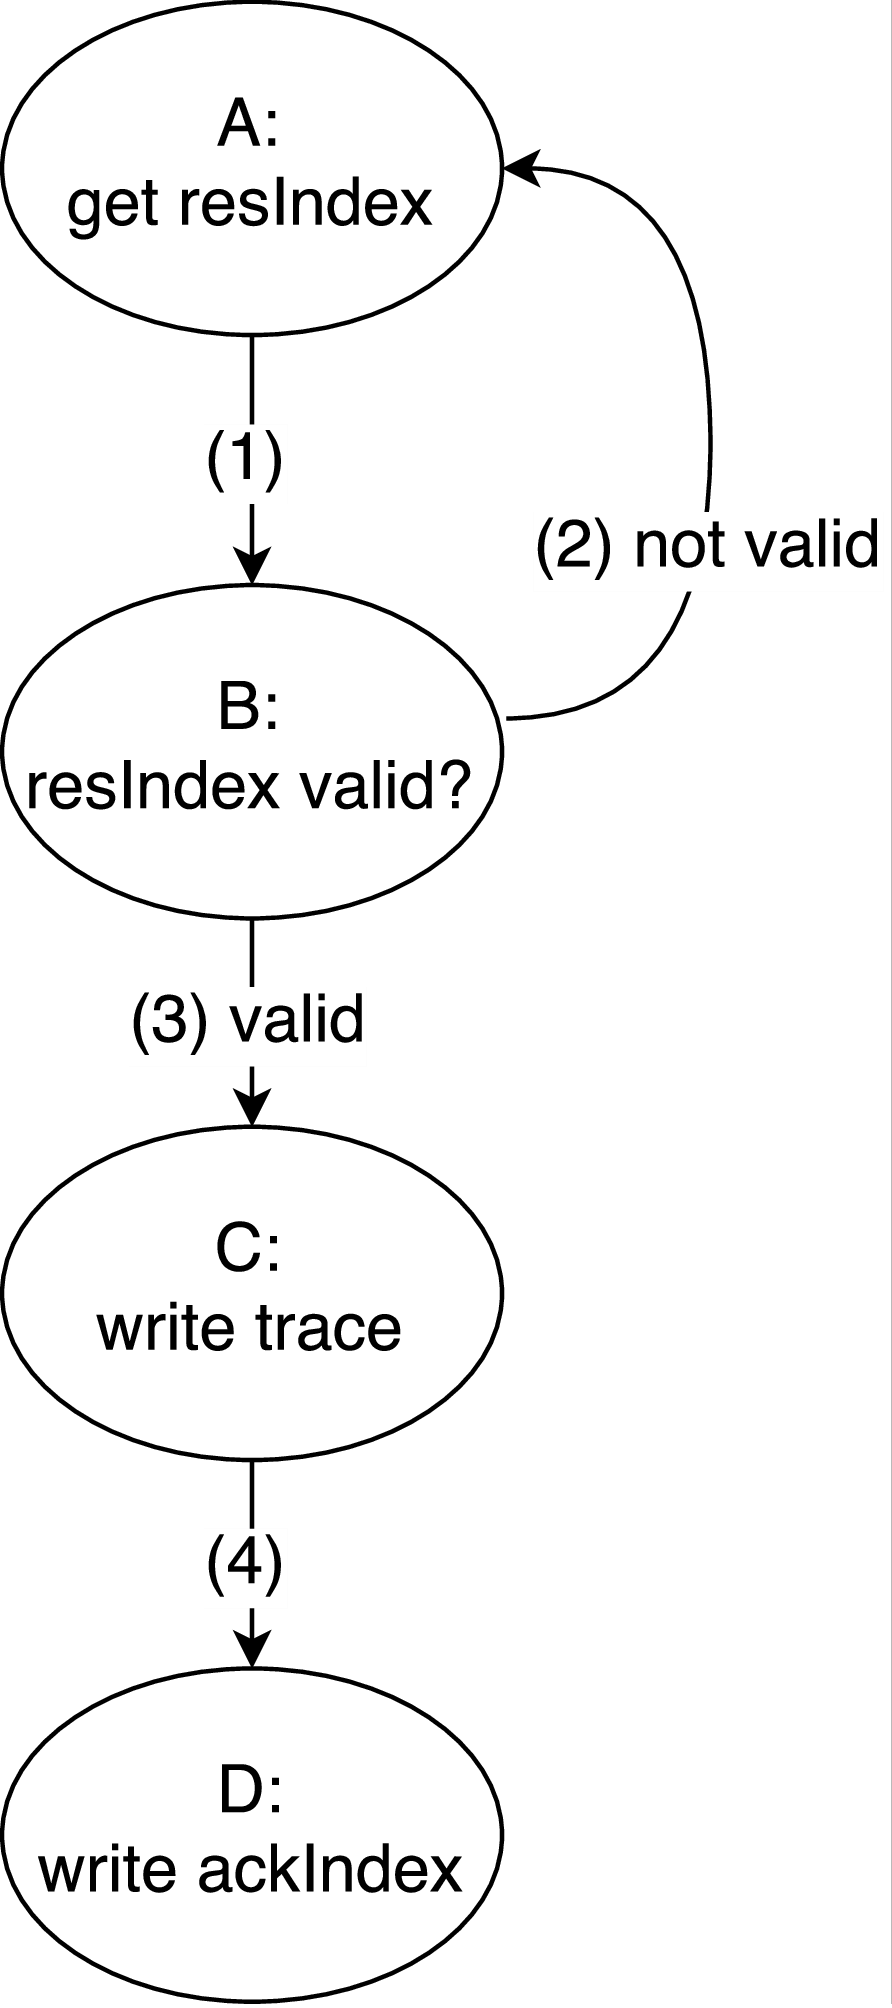
\includegraphics[width=0.3\textwidth]{warp-scope-cfg}
	\caption{Producer CFG}
\label{wscfg}
\end{figure}	
	This section focusses on the producer that is running on the device, making sure that data is only written if there space left
	in a buffer. The producer-consumer setup uses a head and a tail index to handle reservation of buffer space and write acknowledgements to signal that the write has completed. Code sample \ref{prod-cons} shows the pseudo-algorithm that is performed by the producer. First the required buffer space is reserved for writing by incrementing the reservation index
	by the number of required slots (line 1). Then the data generated by the trace is
	written to the buffer (line 2) and the write acknowledgement is incremented by the same number of buffer slots (line 3).
\begin{figure}
	\begin{lstlisting}[style=C]
while((ackIndex > maxIndex) or (id = atomicAdd(resIndex, increment) > maxIndex));
buffer[id] = traceData;
atomicAdd(ackIndex, increment);
\end{lstlisting}
	\caption{Device Producer, naive approach}
	\label{prod-cons}
\end{figure}

	
	This is implemented on a warp scope, which means either the whole warp continues or waits, to prevents deadlocks during indices fetching.
	A deadlock can occur because of how GPUs manage branch divergence inside a warp. If the instruction stream of a warp branches, all member threads of this warp execute both branches, and the group of members that should not be executing this part of the code is masked out. After all branches completed execution, the combined execution of both groups continues.
	
	A deadlock can occur, if each thread fetches it's \verb|resIndex| individually and there is not enough available buffer space for all threads inside the warp. Referring to figure \ref{wscfg} now, all threads will execute edge (1) leading from (A) to (B) by fetching \verb|resIndex|. If all threads get a valid index (B), the warp will not branch and the trace can complete successfully.
	If the check in (B) fails for one or more threads in the warp, a branch is created. The branch without valid IDs will 
	use edge (2), returning to node (A) and retry fetching a valid \verb|resIndex|. The branch with valid \verb|resIndex|
	has to wait with progressing on edge (3) until the group without valid \verb|resIndex| is also ready to continue on edge (3).
	But because the warp can not progress over edge (3) to and C and from there over (4) to D, until all threads have a valid \verb|resIndex|, the threads in the warp that already have a valid \verb|resIndex| can not reach node D write \verb|ackIndex|, which would lead to a evacuation of the buffer on by the host and a reset of the \verb|achIndex| and \verb|resIndex|. As a result of this, a deadlock occurs because one group of threads waits for a resource that can not be released by the other group
	of threads due to the warp execution model.
	
	This can be resolved by handling reservation and write acknowledgement on a warp level. One thread makes the reservation and write the acknowledgement for all threads inside the warp. Now either the whole warp can finish the trace or the whole warp stalls. This way we can use the warp execution model for our purposes, because one thread that waits for the IDs can stall the whole warp with an if branch and no other means of synchronization. This is implemented by using CUDA warp intrinsics, which offer efficient communication inside of warps.
\begin{figure}[t]
	\begin{lstlisting}[style=C]
active   = __ballot(1); // get bitmap of active threads 
nActive  = __popc(active); // get count of active threads
lowest   = __ffs(active)-1; // check which thread has to perform sync
rlane_id = __rlaneid(active, lane_id); // each thread gets its relative Lane id, based on number of active threads
	
if (lane_id == lowest)
	while( ackIndex >= maxIndex-maxWarpWrite 
		|| (id = atomicAdd(resIndex, nActive)) >= maxIndex-maxWarpWrite
	);
// Warp stalls here until all branch is completed

idx = __shfl(id, lowest) + rlane_id; // distribute id
buffer[id] = traceData;
if (lane_id == lowest )
	atomicAdd(ackIndex, n_active);\end{lstlisting}
	\caption{Device Producer, warp scope}
	\label{prod-cons-warp}	
\end{figure}
	Little extra code is needed shift everything to a warp-scope management, as seen in Figure \ref{prod-cons-warp}. Because it is possible that a trace occurs on a point during the execution, where the warp is already branched we have to make sure
	that the indexes are managed correctly and only the currently active threads participate in the trace. The warp intrinsics \verb|__ballot|, \verb|__popc| and \verb|__ffs| are used to determine how many threads are active, and which one has to perform the atomic operations to handle
	the producer synchronization. Then \verb|__rlaneid()|, which is user code, calculates the relative lane id for each warp. 

	While the lowest thread fetches the ID for the buffer using \verb|atomicAdd|, the whole warp stalls at the end of the if clause because of the warp execution model. Once a valid id is fetched, it is distributed among all threads using the \verb|__shfl| intrinsic. 	Then the trace is written and the lowest thread increments the write acknowledgement by the number it increased the reservation.
	
	Notice that in this case, the conditions for fetching the id now takes into account that data is written in blocks and has to check if there is still space left for one complete block. 
	
	Assuming a warp is fully populated warp at the moment a trace happens and thus always reserve enough buffer space for a whole warp can create gaps in the trace data. To prevent old data from lingering, the buffer would need to be wiped after every evacuation of the
	generated trace data. Additionally, these gaps would require additional handling in the analysis of the data.
	Therefore, this more complex approach of handling the consumer was chosen, which only reserved as much space as required.

	
\subsection{Host Consumer}\label{host-cons}
	The consuming thread on the host side is much simpler. A single thread is iterating over all bins in the buffer, checking if the
	\verb|ackIndex| is at the threshold for evacuation. This threshold is reached if there is not enough space for a complete warp to
	write a trace.
	The buffer is evacuated by writing the data into a file handle and \verb|resIndex| and \verb|ackIndex| reset to the beginning of the buffer.

